\subsection{Anonymously Accessing Management Interfaces}

All devices have their \gls{http} Management Interface enabled by default and can be accessed by navigating to \url{http://192.168.15.1} on a browser. This interface provides information about the \gls{cpe} and its network.

On the main page, Figure \ref{figure:main_page_cpe_http_management_interface}, both public and private \gls{ip} addresses of the device can be viewed together with the gateway and \gls{dns} servers configured. The \gls{ssid}, security protocol, \gls{wps} state, and channel of the wireless networks are specified, also showing which \gls{lan} ports are in use. A list with the hostname, \gls{mac} address, and \gls{ip} of all wired and wireless clients currently connected to the \gls{cpe} is present. If \gls{voip} is configured, the telephone number is shown.

\begin{figure}[h]
    \centering
    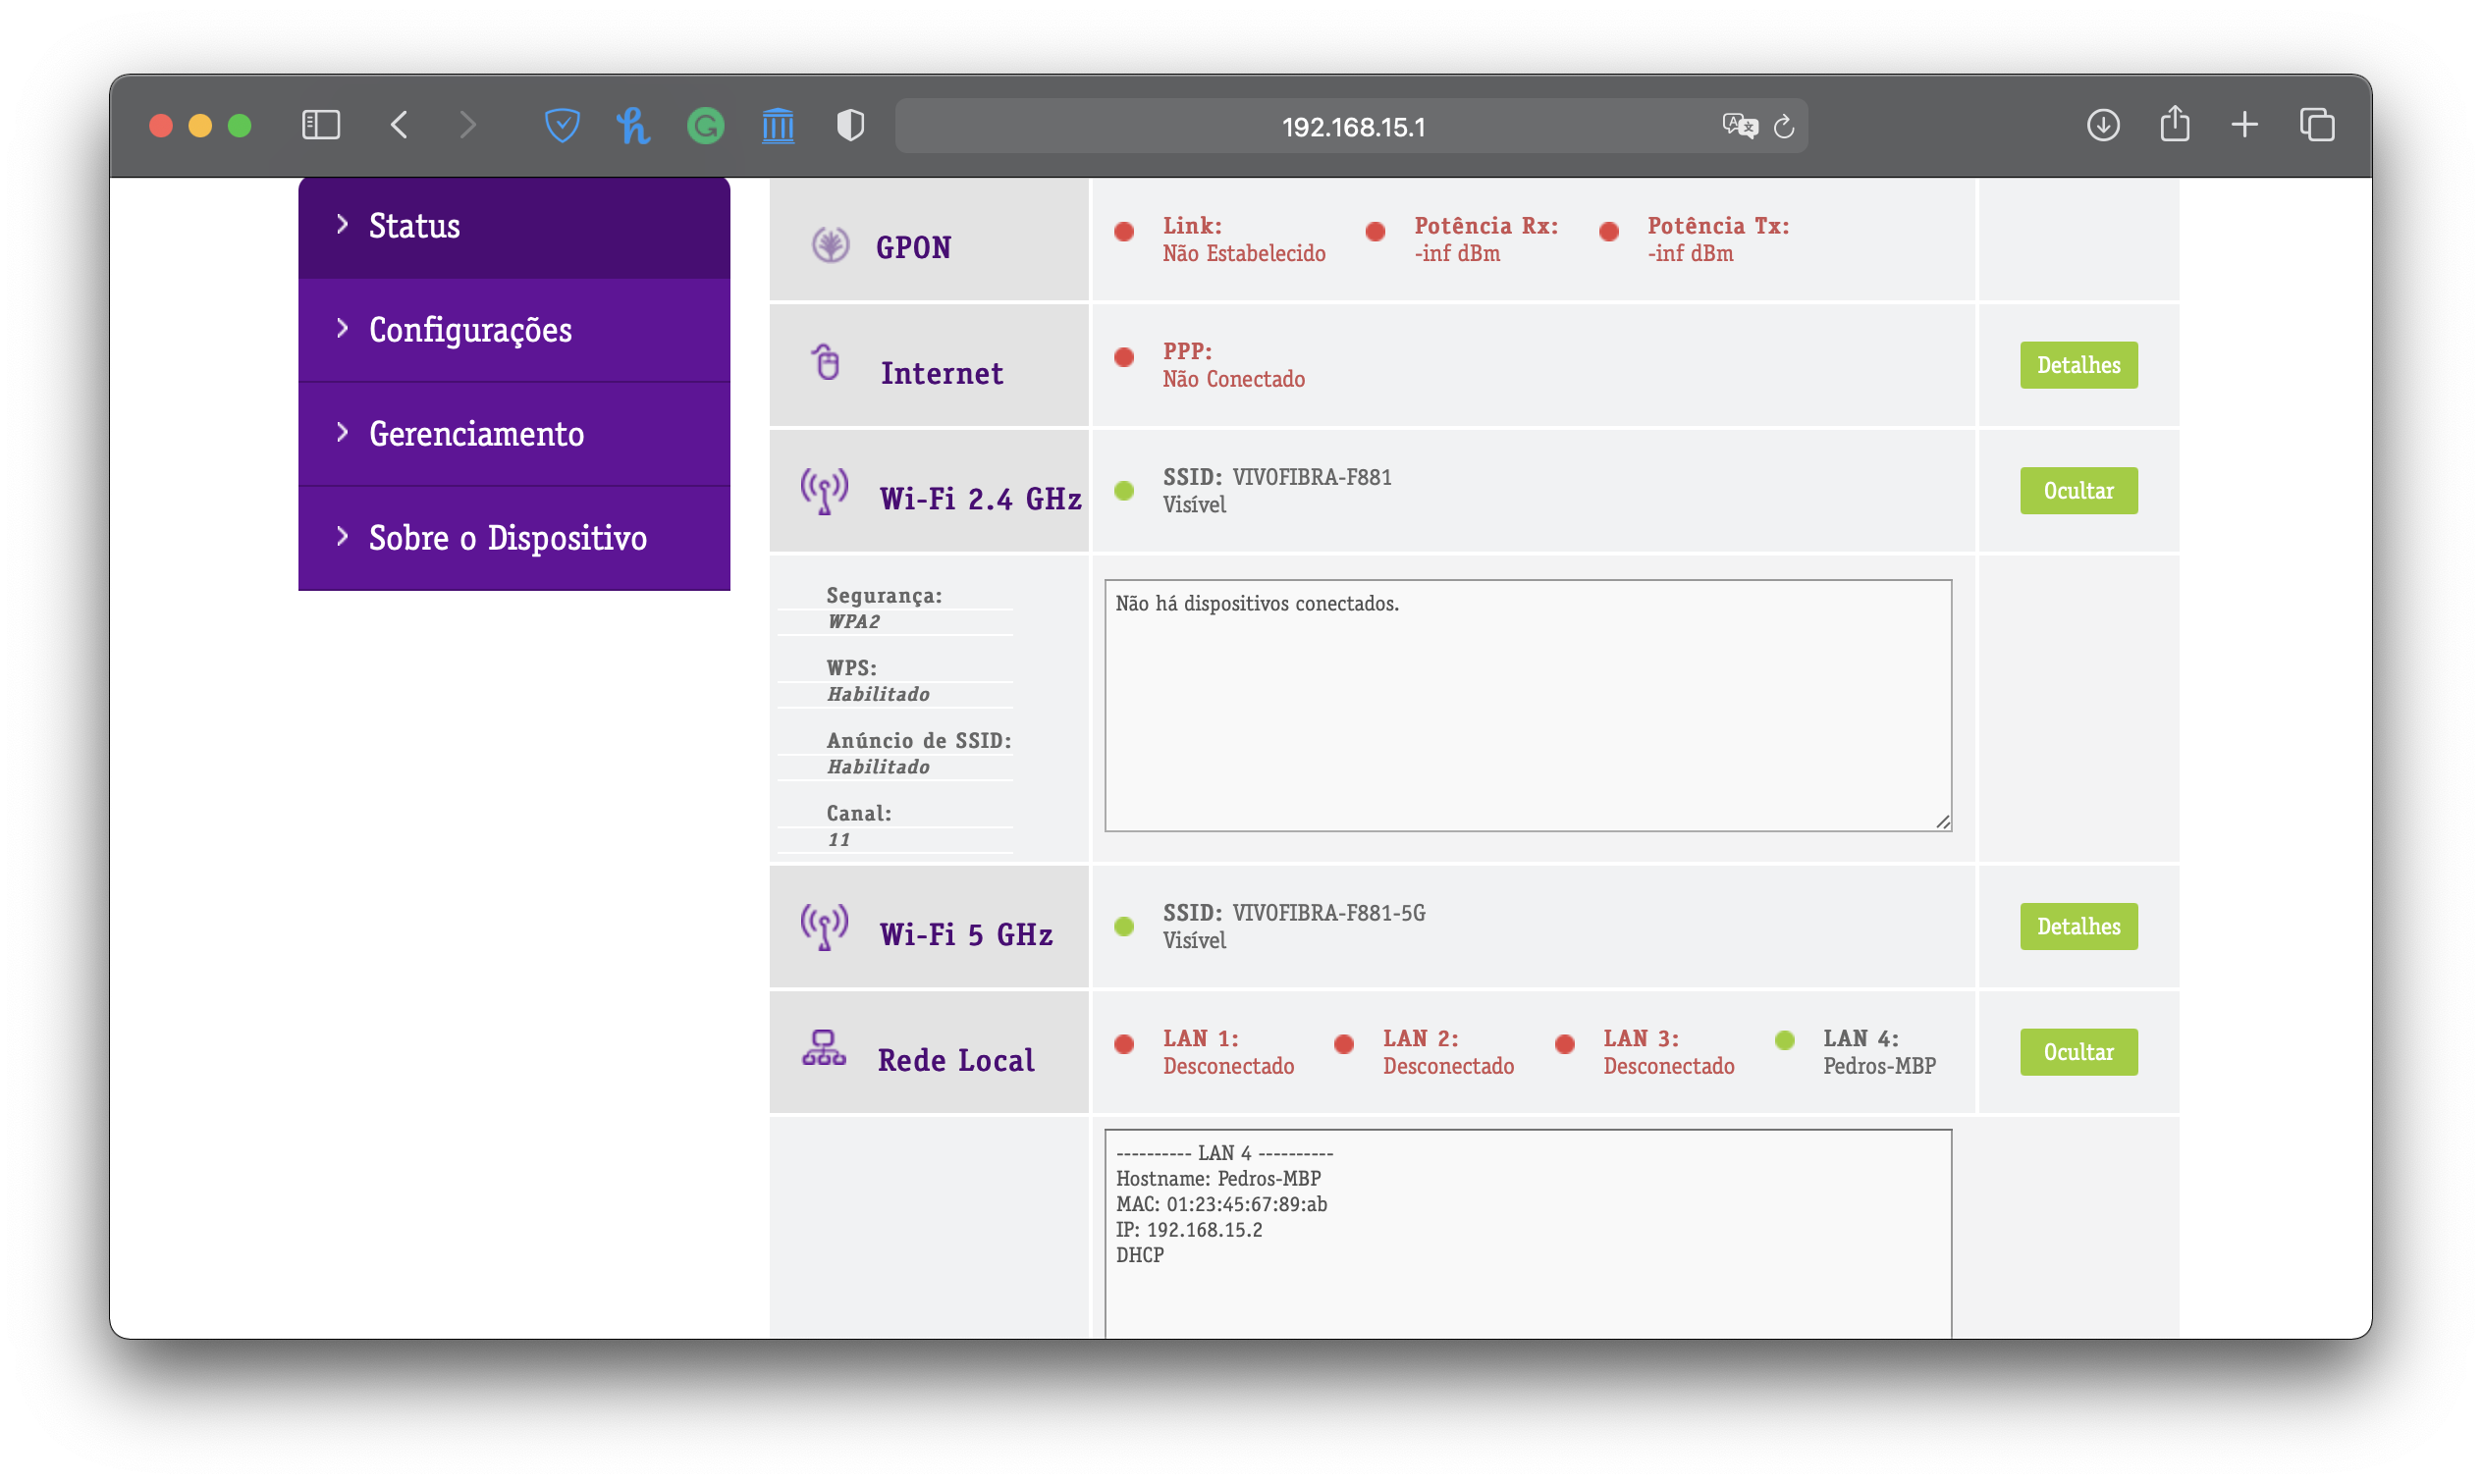
\includegraphics[width=\linewidth]{contents/cpes-and-research-data/anonymously-accessing-management-interfaces/main-page-cpe-http-management-interface.png}
    \caption{Main Page of the \gls{cpe} \gls{http} Management Interface}
    \label{figure:main_page_cpe_http_management_interface}
\end{figure}

The about page of the interface, Figure \ref{figure:about_page_cpe_http_management_interface}, shows the manufacturer, model, firmware version, hardware version, serial number, \gls{wan}-side \gls{mac} address, and \gls{lan}-side \gls{mac} address. If the device is fiber-compatible, it also shows the \gls{gpon} \gls{s/n}.

\begin{figure}[h]
    \centering
    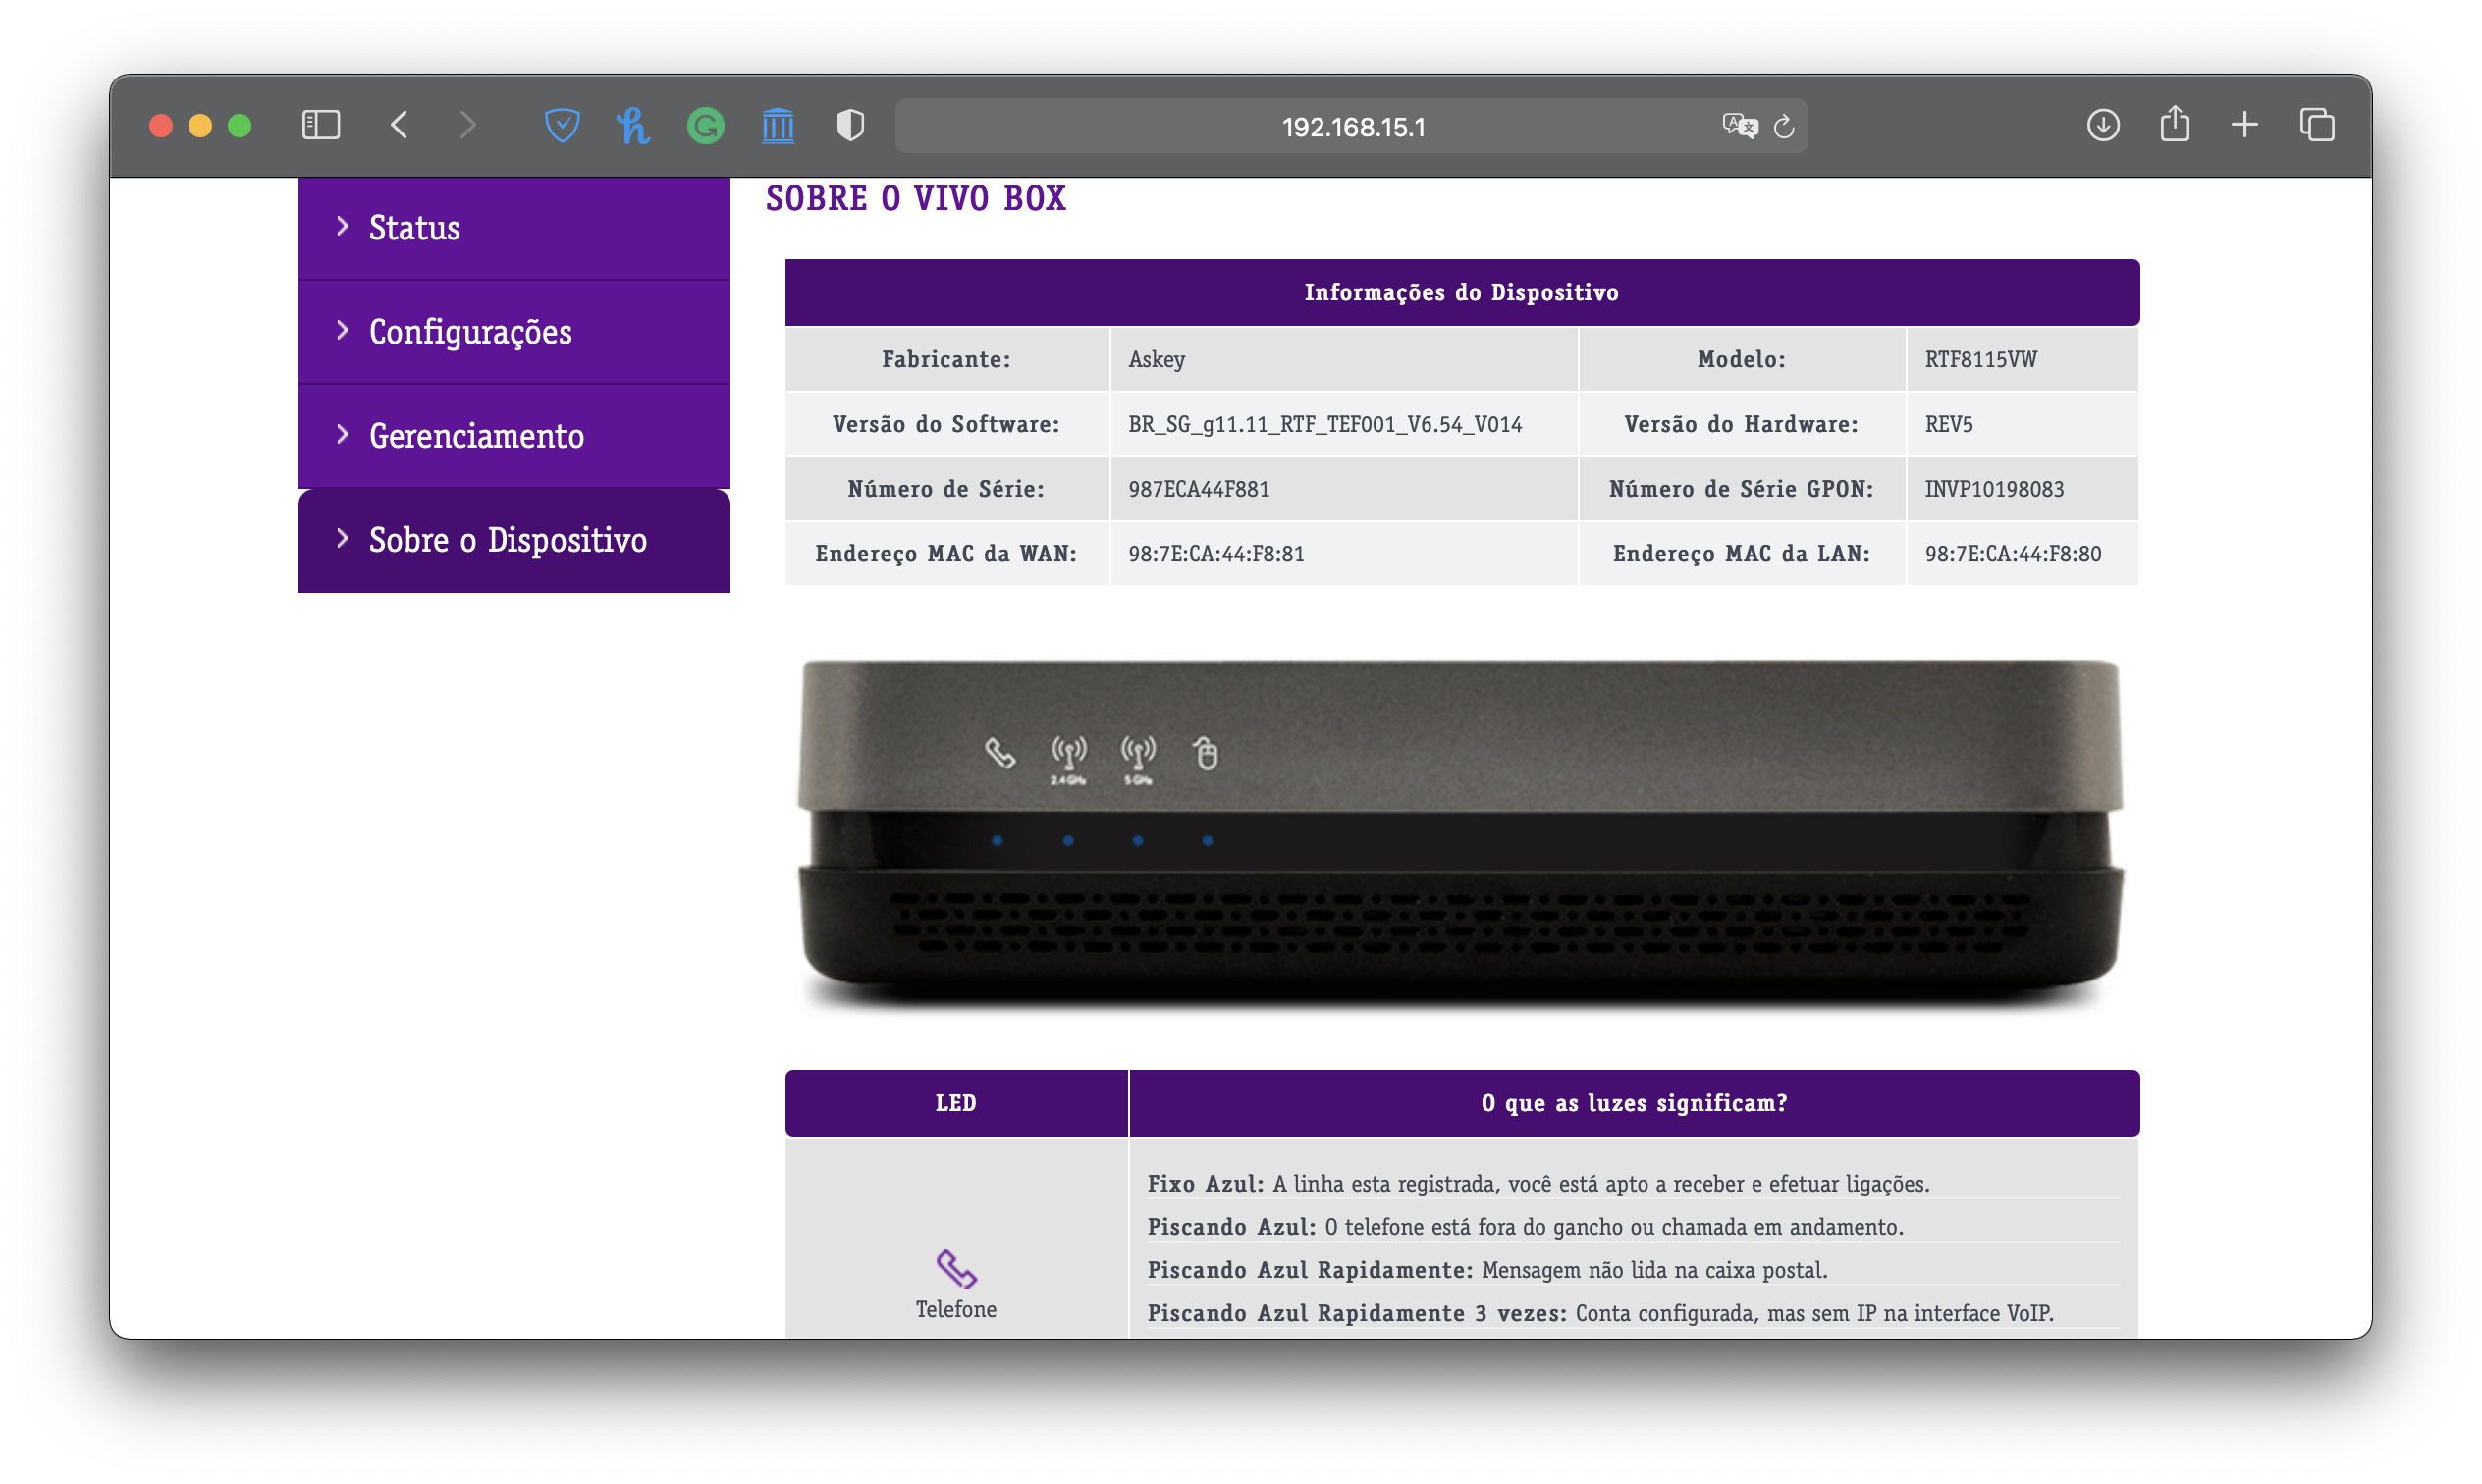
\includegraphics[width=\linewidth]{contents/cpes-and-research-data/anonymously-accessing-management-interfaces/about-page-cpe-http-management-interface.png}
    \caption{About Page of the \gls{cpe} \gls{http} Management Interface}
    \label{figure:about_page_cpe_http_management_interface}
\end{figure}

The \gls{ssh} and Telnet interfaces, even when manually enabled, don’t expose any data about the device without authenticating, immediately requesting credentials.

\FloatBarrier
